\documentclass{Rapport}
\usepackage{RapportFr}

\begin{document}

\chapterN{VoxPopuli: l'interface avec la Régie}	

Les défis proposés par ce projet ne sont pas purement matériels. La gestion du réseau de télécommande nécessite une bonne connaissance du fonctionnement d'un réseau XBee, du protocole de communication utilisé par le calculateur à l'intérieur de chaque télécommande. Bref la gestion bas-niveau du réseau de télécommande ne peut pas être délégué aux concepteurs de "l'application régie" et doit être une composante importante de la solution que nous proposons. 

Le rôle des applications VoxPopuli et de prendre en charge le réseau de télécommande depuis l'ordinateur régie et de proposer des outils de communication fiable et ergonomique pour contrôler ce réseau.

\section{Enjeux du logiciel d'interfaçage}

\subsection*{Fiabilité}
Le premier objectif du logiciel d'interfaçage est sa fiabilité. Bien sur cela suppose qu'il doit planter le moins possible, mais les crashs sont toujours difficile à prévoir (surtout avec un temps de "test" aussi court). En cas de crash il faut donc que le logiciel puisse restaurer l'état dans lequel il se trouvait avant le crash, ainsi le réseau sera en "roue libre" pendant quelques secondes mais retrouvera rapidement son comportement asservie.

\subsection*{Multiplicité de l'interfaçage}
L'enjeux certainement le plus important du logiciel est de pouvoir communiquer avec une ou plusieurs applications desquelles nous ignorons tout, au moment de concevoir l'interface. Le réseau doit pouvoir être accessible depuis les "applications régies" quel que soit le langage dans lequel elles ont été codées. De plus, l'ordinateur de régie doit pouvoir fonctionner sous linux et sous Windows (le logiciel doit pouvoir être executé sur ces deux plateformes).

\subsection*{Ergonomie}
Pour faciliter sa prise en main, le logiciel d'interface doit permettre de controler un réseau à la topologie simple: l'application régie n'a en fait besoin de voir que des télécommandes ou des groupes de télécommandes possédant 5 boutons et 3 LEDs. Toutes informations interne à la gestion du réseau (niveau de batterie ou de signal, état de la télécommande, connexion et déconnexion...) ne doivent pas perturber la clarté de ce réseau simplifier.

Enfin le logiciel doit apporter une solution adapté à l'environnement particulié que constitue le milieu du spectacle: il doit permettre la préparation du spectacle puis sont implantations dans des salles ou des environnements différents.

\pagebreak

\section{Design et philosophie de VoxPopuli}
C'est dans l'optique de satisfaire aux enjeux énoncés plus haut que VoxPopuli a été conçu. Nous aborderons ici les solutions proposées pour répondre à chaque point du cahier des charges.

\subsection*{Fiabilité}
Pour améliorer la fiabilité du logiciel d'interfaçage, les fonctions proposé par VoxPopuli ont été séparées dans deux logiciels distints. Le coeur de l'interface: VoxPopuli Deamon, ne contient que les fonctionnalités de bases. Il est capable de gérer le réseau (connexion, déconnexion), de communiquer avec les applications de régie et de configurer leurs interactions avec les télécommandes. Cependant, il ne possède aucun interface graphique pour limiter les risques de crashs. Ainsi, c'est le deuxième logiciel VoxPopuli GUI qui est chargé de communiquer avec VoxPopuli Deamon et de fournir une interface graphique capable d'afficher, de modifier et de paramétrer le réseau.

En représentation seul VoxPopuli Deamon est réellement utile (puisque toutes les configurations ont normalement été réglées au préalable), c'est donc ce dernier qui dispose d'un mécanisme de récupération de plantage. En pratique, toute les données manipulées par le logiciel durant son execution sont mises en cache sur le disque (leur syntaxe sera executée plus loin dans le rapport). Lorsque le logiciel quitte normalement il vide ce cache, mais lorsqu'il plante ces fichiers restent sur le disque et permettent de restaurer l'état du Deamon lorsqu'on le relance ensuite. Ces fichiers permettent aussi une sauvegarde de la configuration du réseau, en vue de la réutiliser d'un spectacle à l'autre sans avoir besoin de tout reconfigurer.

\subsection*{Multiplicité de l'interfaçage}

Pour répondre au principal défi du cahier des charges, VoxPopuli apporte plusieurs solutions pour interfacer une application avec le réseau de télécommande.

\subsubsection*{Évenements clavier}

La plus simple est certainement d'utiliser les entrées clavier. Il est en effet possible de demander à VoxPopuli Deamon de générer un "faux" évenement clavier (appuie ou relachement d'une touche) lors de l'appuie ou de relachement d'un bouton d'une des télécommandes du réseau. Cette méthode permet un interfaçage simple avec les applications supportant les raccourcis clavier (on peut ainsi controler le défilement d'une présentation power point, jouer aux jeux ne nécéssitant pas de souris, controler un lecteur vidéo...). Cependant, bien que cet interfaçage soit simple à mettre en place, il est à déprécier. En effet, la distribution de l'évenement clavier est déléguée au système d'exploitation qui le transmettra à l'application ayant le focus (en général la fenêtre actuellement sélectionnée). Il est donc impossible de communiquer avec plusieurs applications en même temps et celles-ci n'ont aucun moyen d'action sur le réseau (impossible pour elle d'allumer un LED par exemple).

\subsubsection*{Évenements MIDI et OSC}

Pour établir une communication plus complète entre le réseau et les applications de régie, il faut donc utiliser un vrai protocole de communication entre applications. Ils existent de nombreux protocoles différents pour réaliser cette tâche. Nous avons donc sélectionnée ceux les plus utilisés dans le milieu du spectacle. VoxPopuli peut ainsi générer et recevoir des évènements MIDI (Musical Instrument Digital Interface) et sa version améliorée OSC (Open Sound Control). Tout comme les évènements clavier, on peut configurer le logiciel pour qu'il fasse correspondre un évènement MIDI ou OSC à un changement d'état d'un bouton d'une télécommande, mais il est aussi possible de contrôler la puissance de LED via ces protocoles. Et contrairement à l'interfaçage clavier, il est possible de paramétrer plusieurs ports MIDI ou OSC, pour chacune des applications régies.

\subsubsection*{CLI via telnet}

Enfin une dernière solution de communication  a été mis en place. En effet, malgré l'efficacité du MIDI et de l'OSC pour controler le réseau pendant la représentation, ces protocoles se montrent parfaitement inadaptés pour configurer VoxPopuli Deamon. Pour combler cette lacune, VoxPopuli Deamon dispose d'une Interface en Ligne de Commande (CLI) disponible via telnet. Cette interface en ligne de commande permet d'accéder à la totalité des fonctionnalités du logiciel d'interfaçage que ce soit pour configurer et surveiller le réseau de télécommande ou paramétrer les interactions avec les différentes applications régies. Le fonctionnement de cette CLI sera détaillé plus loin dans ce rapport. C'est l'interface à privilégier pour le paramétrage du réseau (c'est celle utilisée par VoxPopuli GUI pour communiquer avec VoxPopuli Deamon), et elle peut aussi être utilisée pour relayer les évènements provenant ou à destination des télécommandes (même si elle possède une latence légèrement supérieure par rapport au MIDI).

\subsubsection*{Fichiers de cache}

Une dernière solution existe pour configurer VoxPopuli Deamon: modifier directement les fichiers mis en cache sur le disque qui décrivent la totalité des variables manipuler par le logiciel. Cette méthode est cependant déconseilée à moins d'être sur de la syntaxe  de ces fichiers.

\subsubsection*{En bref}

Le schéma suivant présente tous les interfaçages possible du réseau:

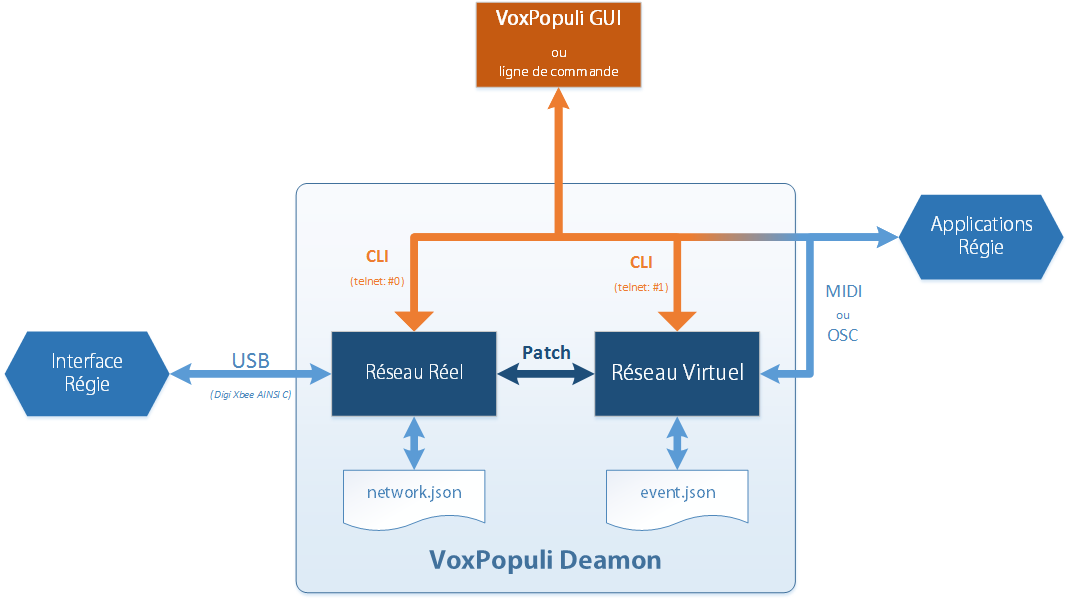
\includegraphics[width=0.8\columnwidth]{rsc/diaGeneral}

\subsection*{Ergonomie et simplicité d'utilisation}

En vu d'être utiliser dans le contexte d'un spectacle, VoxPopuli Deamon propose une architecture qui permet à la fois de configurer et de tester le réseau de télécommande sans avoir besoin d'installer toutes les télécommandes, mais aussi de pouvoir adapter une installation de télécommande propre à une représentation à la configuration réalisée.

Pour ce faire, le réseau "physique" (ou réel) de télécommande est découplé du réseau "virtuel" qui communique avec les Applications Régies. Lors de la conception du spectacle, on définit des télécommandes virtuelles et on configure les évenements qu'elles enverront ou pourront recevoir durant la présentation. Ces interactions peuvent alors être simulée sans avoir recours à une vrai télécommande. Au moment de l'installation des télécommandes dans la salle de spectacle chacune d'entre elle devra être connectée à une télécommande virtuelle et toute les interactions de la deuxième seront alors répercutées sur la première. Ces connexions sont réalisées au moyen d'un patch interne à VoxPopuli Deamon.

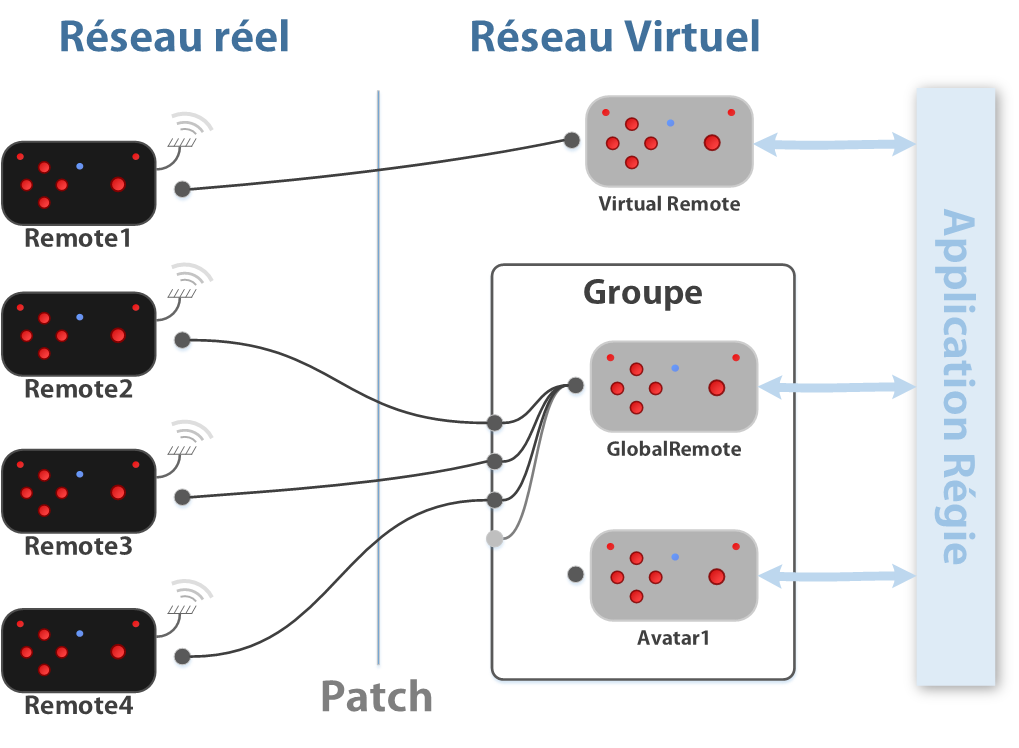
\includegraphics[width=0.8\columnwidth]{rsc/diaReseau}

À ce mécanisme de patch s'ajoute la possibilité de définir Groupe dans le réseau virtuel. Un groupe virtuel permet de gérer un ensemble de télécommande sans connaître leur nombre à l'avance. Vu du réseau réel, un groupe peut être connecté à plusieurs télécommandes réelles, vu de l'application régie il permet de modifier l'état de  toutes les télécommandes simultanément via la télécommande virtuelle GlobalRemote, ou bien d'une en particulier via des télécommandes "avatars". En effet, les télécommandes virtuelles avatars peuvent être dynamiquement (et même aléatoirement) connectées à une des télécommandes réelles du groupe, mais offre une interface constante aux applications de régies. 

Quelles opèrent en solitaire ou au service d'un groupe les télécommandes virtuelles ont ainsi toujours les mêmes contrôles évenementiels:

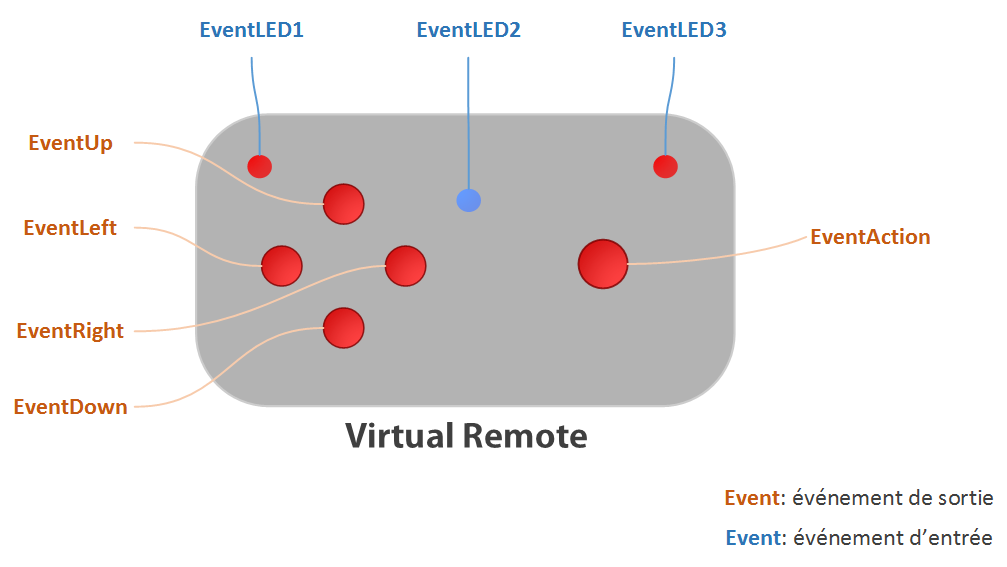
\includegraphics[width=0.8\columnwidth]{rsc/diaVirtualRemote}


Dans le cas d'une "histoire simple", les télécommandes de chaque écrans ont tout intérêt à être placées dans un groupe. Pour les séquences de vote, un controle de toutes les télécommandes en simultané peut-être suffisant, puis pour les séquences de jeu il suffit de demander à une télécommande avatar de se connecter à une seule télécommande réelle du groupe. L'interfaçage avec le jeu est alors simple puisque quelque soit la télécommande réelle choisie, les évenements envoyés par l'avatar seront les mêmes.


\section{Syntaxe de communication}

La configuration du réseau consiste donc en une communication avec VoxPopuli Deamon qui passe soit par la modification des fichiers de caches du logiciel, ou par la CLI via telnet. Nous présenterons ici la syntaxe générale choisie pour ces deux communications.

\subsection*{Le format JSon}
Le format choisit pour la sauvegarde du modèle dans les fichiers de cache est le JSon. Ce langage descriptif, extension du javascript, permet de décrire une arborescence d'objet (comme l'XML) tout en restant facilement lisible par un humain.

En JSon, un objet est défini par un ensemble de propriétés chacune définie par un nom et une valeur. Cette valeur peut être de type:
\begin{itemize}
	\item chaine de caractère
	\item nombre
	\item booléen
	\item tableau de valeur (pas forcément toutes du même types)
	\item objet
\end{itemize}
Les objets étant acceptés comme propriétés, le JSon permet de définir des arborecences.

Au niveau de la syntaxe les propriétés sont définies par leur nom entre guillemets, de deux points puis de leur valeur:
\sample{"nom": valeur}

Les tableaux sont définis entre crochets, chacune de leur valeurs étant séparée par une virgule.

Enfin, un objet commence par une accolade ouvrante et se termine par une accolade fermante, chacune de ses propriétés est séparée d'une virgule:
\sample{\{\\
\tab	"Propriété1": 1,\\
\tab	"Propriété2": "valeur",\\
\tab	"Tableau": ["valeur",1,true]\\
\}}

Il est important de noter que la totalité des informations manipulée par VoxPopuli Deamon sont stockées dans des modèles suivants cette syntaxe. Pour marquer la séparation entre réseau physique et réseau virtuel et pour pouvoir les enregistrer et recharcher séparément, chacun possède son modèle JSon propre. Ainsi toutes les informations concernant le réseau réel sont-elles stockées dans le fichier "network.json" et celles concernant le réseau virtuel dans "event.json".  Les propriétés définies par ces modèles sont détaillées plus loin dans le rapport.

\subsection*{Interface en Ligne de Commande via telnet}
La CLI est accessible via telnet sur le port 9000 de l'ordinateur de régie (elle est accessible depuis n'importe quel terminal du réseau si le par-feu de l'ordinateur régie l'autorise). Les commandes interprétées par la CLI sont de deux types: les commandes de configuration de la CLI qui commencent toutes par \verb|#|, et les commandes destinées aux modèles JSon.

Pour modifier les propriétés d'un modèle JSon via telnet, il faut d'abords sélectionner ce modèle grâce à la commande \verb|#0| pour network.json ou \verb|#1| pour event.json. Une fois le modèle sélectionné, toutes ses propriétés sont accessible à la lecture. Il suffit de taper leur adresse pour en connaitre leur valeur. L'addresse d'une propriété est constitué par la suite de noms des noeuds qu'il faut parcourir pour l'atteindre, les noms étant séparés par des points.

Ainsi pour le modèle json suivant:
\begin{Cpp}
{
	"Remotes": {
		"Remote1": {
			// ...
			"LED1": 0,
			// ...
		}
	},
	"USBPort": "/dev/ttyUSB0"
}
\end{Cpp}

On peut récupérer la valeur de la LED de la télécommande 1 par la commande (le \verb|>| est afficher par la console telnet quand celle-ci écoute):

\sample{>Remotes.Remote1.LED1\\
	Remotes.Remote1.LED1: 0}

De la même manière on peut modifier la valeur d'une propriété du modèle en ajoutant à son addresse deux points puis sa nouvelle valeur. Il faut tout de même noter que toutes les propriétés du modèle ne peuvent pas être modifier depuis la CLI (par exemple le niveau de batterie d'une télécommande...). Pour allumer la LED de la télécommande 1 au maximum, il faut donc entrer la commande:

\sample{>Remotes.Remote1.LED1: 254}

Il est possible de demander à la CLI d'afficher toute modification du modèle JSon et ce, quelque soit la provenance de la modification. Pour ce faire il faut configurer la CLI en mode verbose par la commande: \verb|#v| (et \verb|#-v| pour en sortir). Ce mode permet de synchroniser en permanence l'état du modèle manipulé par VoxPopuli Deamon.

Enfin les objets des modèles JSon disposent de méthodes qui peuvent être appelées par la CLI de la même manière que les propriétés. Ainsi tous les objets disposent d'une méthode \verb|print()| qui affiche leur contenu en format JSon. Certains objets (comme les télécommandes) peuvent être renommé par la méthode \verb|rename( "nouveauNom" )|.

Ainsi pour renommer \verb|Remote1| en \verb|Telecommande1| il faut executé la commande:
\sample{>Remotes.Remote1.rename("Telecommande1")\\
Remotes.Remote1 renamed "Telecommande1"	}
La réponse renvoyée par la CLI stipulant que l'opération de renommage s'est déroulée correctement ne s'affiche qu'en mode verbose.

%\section{Détail des modèles JSON}
%
%La syntaxe décrite plus haut définit un cadre, une architecture dans laquelle il faut préciser le détail de chaque modèle. On s'attardera ici sur la définition de tous les objets qui peuvent apparaitre dans le modèle network.json et event.json. Pour chacun d'entre eux on étudiera leur valeur par défaut, les méthodes qu'ils mettent à disposition et les propriétés qu'ils contiennent.
%
%\subsection*{network.json}
%
%\subsubsection*{Modèle par défaut}
%\begin{Cpp}
%{
%	"Patch":
%	{	
%	},
%	"Remotes":
%	{	
%	},
%	"USBPort": ""
%}
%\end{Cpp}
%
%\subsubsection*{Méthodes}
%
%\textbf{listPort()}: liste les ports USB connectés à une liaison série (potentiellement le coordinateur du réseau).
%
%\textbf{scan()}: scanne le réseau pour détecter les nouvelles télécommandes.
%
%\textbf{sendAT()}: envoie une commande AT à la carte XBee coordinatrice du réseau
%
%\subsubsection*{Propriétés}
%
%\textbf{USBPort}: Le port série sur lequel VoxPopuli Deamon doit se connecter
%
%\textbf{Remotes}: Une liste d'objets de type \verb|Remote| qui représentent les télécommandes réelles du réseau.
%
%\textbf{Patch}: Liste de connexion entre les télécommandes réelles et les télécommandes ou groupes virtuels.
%\subsubsection*{title}
%
%\subsection*{event.json}
%


%\section{Implémentation}
%Ce rapport n'a pas vocation à décrire l'implémentation de VoxPopuli de manière exhaustive, cette section à simplement pour objectif de permettre au lecteur de se plonger dans le code sans s'y noyer. 
%\subsection*{Organisation du code}
%\subsection*{Librairie utilisée}
%\subsection*{Articuler un model JSon}
%\subsection*{Gestion du multithread}

\end{document} 	
